\chapter{ Констукторский раздел}
\label{cha:design}

Ниже представлены схемы алгоритмов -- Дамерау - Левенштейна и двух реализаций Левенштейна(рекурсивный и обычный).

\section{ Разработка алгоритмов}
\subsection{ Расстояние Левенштейна(обычный)}

\begin{figure}[ht!]
    \centering{
        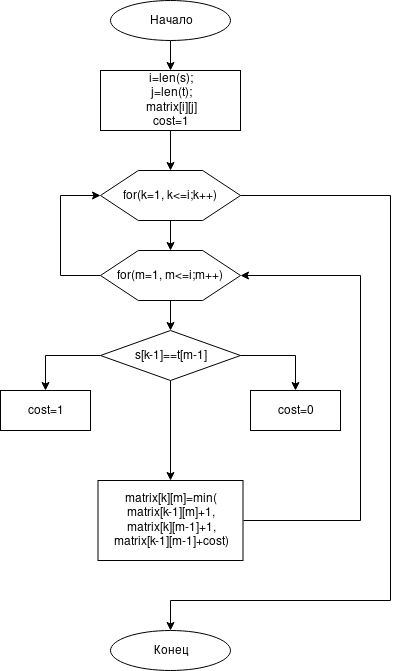
\includegraphics[width=0.4\textwidth]{img/levenstein.png}
        \caption{ Представлена схема алгоритма нахождения расстояния Левенштейна для матричной реализации}}
\end{figure}

\subsection{ Расстояние Дамерау -- Левенштейна}

\begin{figure}[ht!]
	\centering{
        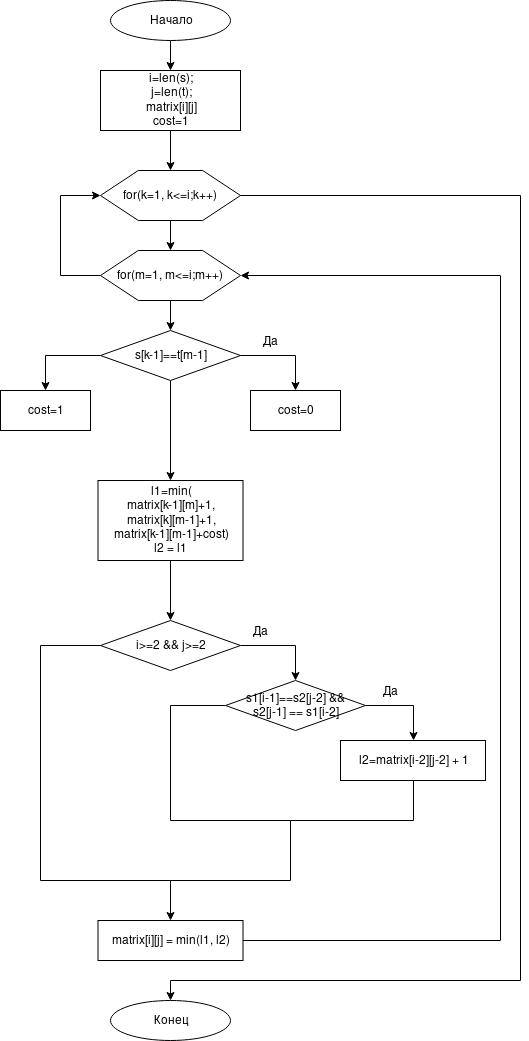
\includegraphics[width=0.4\textwidth]{img/damerau_levenstein.png}
        \caption{Представлена схема алгоритма нахождения расстояния Дамерау -- Левенштейна для матричной реализации}}
\end{figure}
